\chapter{Interactive Feature Selection Design}
In this section, we outline the design goals of our system and describe the design of each component and interaction. The system's workflow for collaborative feature selection is derived from the analysis of feature selection techniques and ideas on how to incorporate humans into the techniques. We describe each step of the process and explain how each step supports collaborative feature selection. We also describe how the overall system supports iterative predictive modeling and how to compare different models.

\section{Design Goals}
The first design goal of the system is to facilitate collaboration between the user and machine at performing feature selection. The second design goal is to design interactions and visualizations that support efficient and effective communication. Lastly, the system is designed to establish and incorporate prior knowledge which would support the user at filtering features. Feature relevance and causal relationship are two types of prior knowledge that we identified and integrated into the system. The system is designed such that we can easily integrate another step in the workflow to capture other aspects of prior knowledge. 

\subsection{System Overview}
We devise a workflow for collaborative feature selection. The steps of the process are expressing feature importance, expressing causal relationships, exploring feature sets and creating a model, and analyzing and comparing model performances. We first acquire prior knowledge from the user and integrate that information into the rest of the workflow. The purpose of the first two steps, expressing feature importance and expressing causal relationships, is to acquire prior knowledge. In the next step, the user interactively explores the feature space and the system assesses how consistent the feature set is in relation to the previously provided information. Then a model is built using features manually filtered by the user. Lastly, the user evaluates and compares the performances of different models.

Separate interfaces and interactions are designed for each step. The steps are chronologically outlined at the top of the interface and the current step is highlighted. 

\section{Expressing Feature Importance}

\begin{figure}[!htbp]
\centering
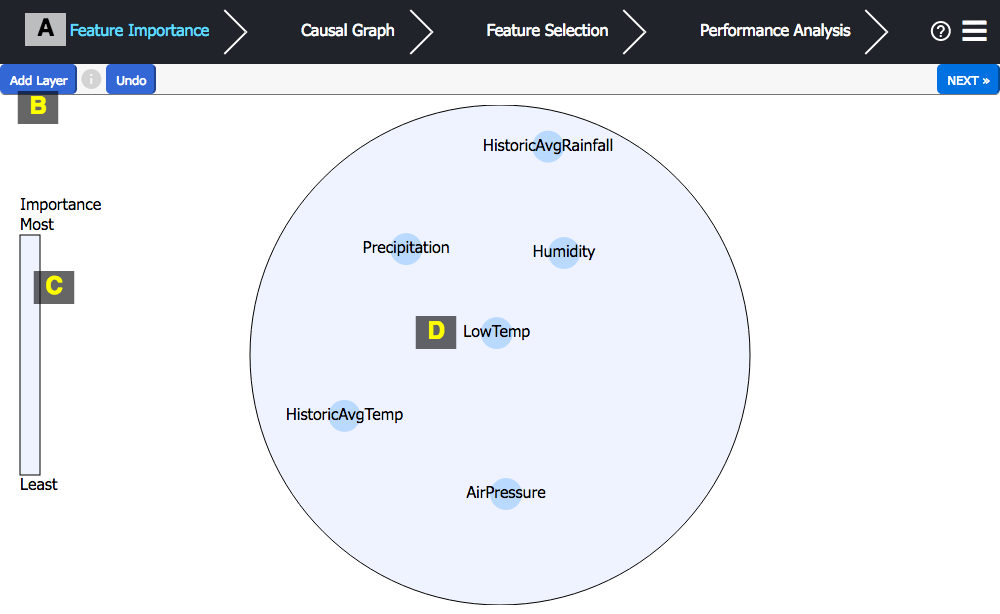
\includegraphics[width=1\textwidth]{InitialUserInterface}
\caption{\textbf{Initial User Interface for Expressing Feature Importance}. The classification task in the following figures is predicting tomorrow's weather conditions based on today's weather metrics. (A) The steps of the feature selection process are outlined horizontally at the top of the interface. (B) The user can click the 'Add Circle' button to create an additional inner circle that will represent a grouping of features with about the same level of importance. (C) A legend correlates the color of a circle to its relative level of importance. (D) Concentric circles are used to visually express the different levels of feature importance at predicting the target. }\label{fig:InitialUserInterface}
\end{figure}
 
\begin{figure}
    \centering
    \begin{minipage}{0.5\textwidth}
        \centering
        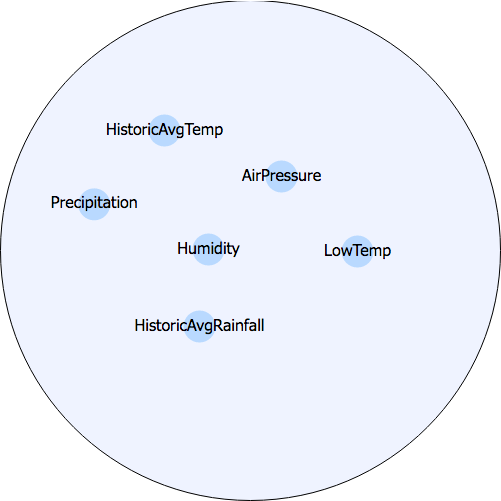
\includegraphics[width=0.825\textwidth]{FeatureImportance1}
    \end{minipage}\hfill
    \begin{minipage}{0.5\textwidth}
        \centering
        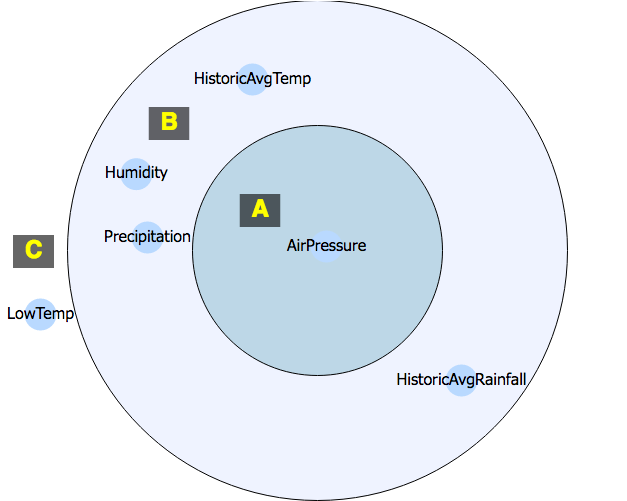
\includegraphics[width=1\textwidth]{FeatureImportance2Labeled}
    \end{minipage}
    \caption{\textbf{Express Feature Importance.} (Left) Initially, all features are grouped in the same circle to express that they are equally important at predicting the target (Right) (A) Air pressure is most relevant or important feature for predicting weather condition (B) The user does not know whether historical average temperature, humidity, precipitation, and historical rainfall are relevant to tomorrow's weather condition or the user does not think those features are as important as air pressure. (C) Today's recorded low temperature is not relevant to the classification task.}
    \label{fig:ExpressFeatureImportance}
\end{figure}

The user often has a rich knowledge of the problem background and feature semantics that the feature selection algorithms do not know about. The first step enables the user to visually express their prior knowledge about the importance or relevance of features at predicting the target label. The motivation is to integrate the user's prior knowledge as a criterion for filtering features. 

As shown in figure \ref{fig:InitialUserInterface}, the system represents features as labeled nodes and uses concentric circles to represent a ranking and grouping of importance. Features placed in the same circle are equally important. Initially, the system has no information about feature importance, and all features are grouped inside one large circle to represent that they are equally important at predicting the target label (figure \ref{fig:ExpressFeatureImportance}). If the user has no background information about which features may be relevant to the target, the user can move onto the next step without interacting with the visual. 

Otherwise, the user can interact with the visual to express which features are relevant, more relevant than others, or irrelevant. To express that a feature is more relevant than others, we distinguish the feature by placing it in a different group. We click the ``Add Circle" button to add an inner circle which represents a group of more relevant features. We leave the features that are either less relevant or we have no prior knowledge about in the outermost circle. In addition, we indicate a feature is irrelevant by moving it outside of the circles or groups as shown in figure \ref{fig:ExpressFeatureImportance}. 

Moreover, we can order features in terms of relevance. The user may have evidence that a feature may be predictive of the target, but the feature may not be as predictive or the user may not be as certain about its relevance compared to features in the innermost circle. To express this, the user can add another concentric circle and place features into the second most inner circle as shown in figure \ref{fig:FeatureImportance3}. Therefore, the groups of features also represent an ordering of feature importance. The user can continue to add inner circles to represent a group of features with the same level of importance and express a group's importance relative to the other groups. 

\begin{figure}[!htbp]
\centering
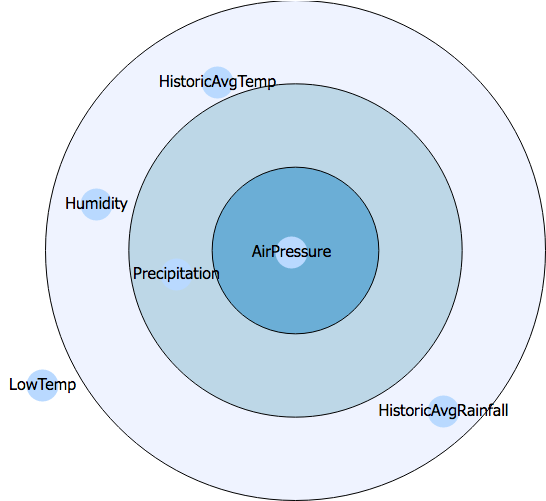
\includegraphics[width=0.65\textwidth]{FeatureImportance3}
\caption{\textbf{Ordering Feature Importance.} Air Pressure in the innermost circle is the most relevant feature. Precipitation in the second inner circle is more relevant than the features in the othermost circle but less relevant than air pressure.} \label{fig:FeatureImportance3}
\end{figure}

The interface is designed to help users visually translate their prior knowledge. The coloring of the concentric circles is a gradient. Humans are visually biased towards darker colors representing more. So the innermost circle is colored the darkest blue to represent the group with most relevance, while the outermost circle is the lightest blue to represent the group with the least relevance. Irrelevant features are placed in a white background, reinforcing that these features do not relate to the features in the colored circles. The gradient coloring of the concentric circles also corresponds to the ordering of feature relevance, and the color helps reaffirm the importance of features grouped in the circle.

When the user explores the feature space, the consistency of a feature set in relation to feature importance is quantified to help the user assess the feature set. The system treats the feature importance ordering and feature selection as rankings and measures consistency using rank loss. The feature importance visual can be translated to a ranking where more important features have higher ranks. The most important features in the innermost circle have the highest possible rank of 0. The immediate outer circle has a rank of 1; rank increments by one as we move towards outer circles, and features outside of the concentric circles are given the lowest rank. Feature selection can also be described as a ranking function, where selected features have the highest rank of 0 and not selected features have a rank of 1. The ranking function for feature selection, where $S$ is the set of selected features, is 
\begin{equation}
  f(x) =
    \begin{cases}
      0 & \text{if $x \in S$}\\
      1 & \text{otherwise}
    \end{cases}       
\end{equation}

Feature selections are converted to rankings and compared against the feature importance ranking. A list-wise approach is used to calculate the rank loss between the feature selection ranking function and feature importance rank list. 
\begin{equation}
\label{eqn:rankloss}
L(f; X, y) = \sum_{s=1}^{n-1}(-f(x_y(s)) + ln(\sum_{i=s}^{n}exp(f(x_y(i)))))
\end{equation}
where \(X = {x_1,..., x_n}\) is the feature vector to be ranked and \(y\) is the feature importance ranking list \cite{RankLoss}. 
A feature set that minimizes rank loss is more consistent with the feature importance ranking. However, noted that all the features are ranked 0 by default when the user does not have prior knowledge about relevance; therefore, \(L\) equals 0 for all possible selected feature sets. Although in this case, the rank loss does not help discover predictive feature sets, the system is designed to be used for classification problems where the user has prior knowledge to contribute. 

\section{Expressing Causal Relationship}
\begin{figure}[!htbp]
\centering
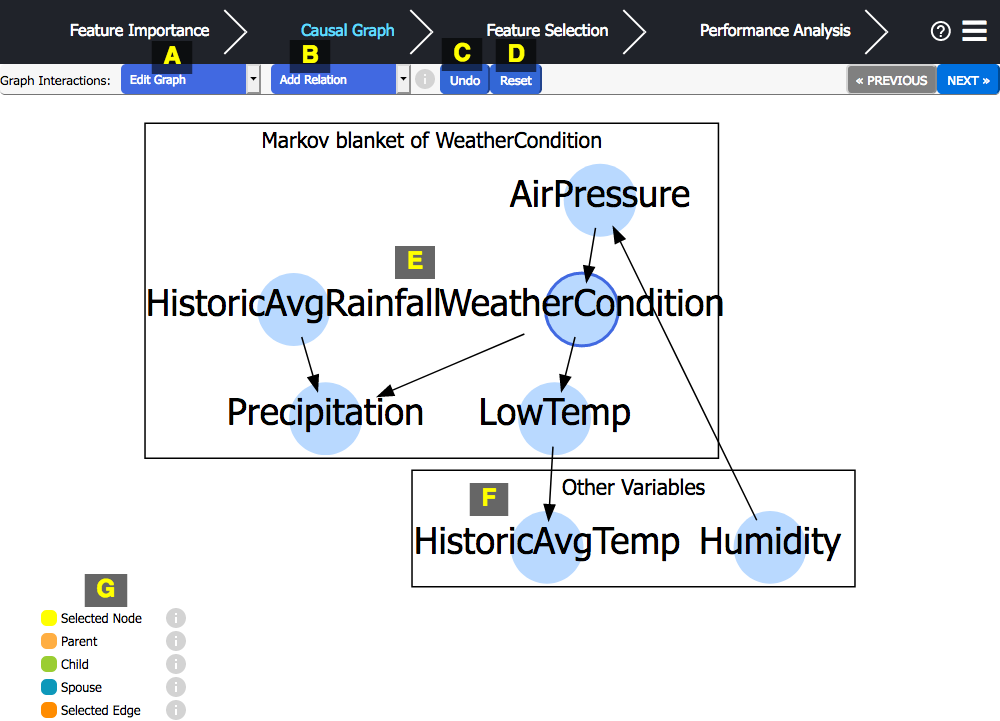
\includegraphics[width=1\textwidth]{LabeledCGInterface}
\caption{\textbf{Expressing Causal Relationship Interface.}  (A) User can select how to interact with the graph. The two graph interaction options are ``Highlight Selected" and ``Edit Graph". (B) The user can choose to highlight the selected feature's Markov blanket or its paths to/from the target. The user can edit the graph by adding an edge, removing an edge, reversing an edge, or removing a feature. (C) The user can undo graph edits. (D) The user can reset the graph to the original. (E) The interface shows a possible causal network fitting the weather condition dataset. The target variable, weather condition, and its Markov blanket features are outlined to highlight a predictive feature set based on causality. (F) The other features are grouped in a different subgraph. The edges between the subgraphs show which non-Markov blanket features are affected by or effect Markov blanket features. For example, the non-Markov blanket feature, historical average temperature is affected by low temperature. (G) The color of the highlighted features indicates their relationship to the selected feature. Initially, no feature is selected.} \label{fig:LabelCGInterface}
\end{figure}

As described in section \ref{CausalFSSubsection}, research has shown that feature selection techniques benefit from the integration of causality. In the second step, the system constructs a causal network that fits the dataset and also represents prior knowledge the user may have about cause and effect relationships in the dataset. We include information about feature importance in the causal discovery algorithm. Moreover, we seek help from the user at modifying the graph. The motivation for the second step is to interactively construct a graph that represents possible causal relationships and also is reflective of the user's prior knowledge. Causality is then incorporated as a filter criterion for feature selection.

Since causal discovery is not the primary contribution of this project, we designed the system to be agnostic to causal discovery algorithm. We integrate a causal discovery library, PyCausal, implemented by the Center of Causal Discovery rather than implement an algorithm ourselves. We use Greedy Equivalence Search (GES), a causal discovery algorithm described in subsection \ref{GESSubsection}, to build an initial causal network fitting the observed data. We can replace GES with another causal discovery algorithm without affecting the interface and functionalities.

We designed the system to build upon previously expressed prior information. For example, we incorporate feature importance as prior to the network. We impose direct dependencies between highly relevant features and the target variable. The algorithm will output a network containing direct edges between the highly relevant features and target. The direction of dependence is not imposed since we assume both direct cause or direct effect are highly relevant. Similarly, we impose independencies between the irrelevant features and target variable, and so irrelevant features do not directly connect to the target in the output network. The user is allowed to go back and modify feature importance. Since the causal graph depends on the information provided at the feature importance step, the causal graph is rebuilt when feature importance changes.

The causal relationships discovered by the algorithm are represented in a Bayesian network described in section \ref{CBN}. The graph is modified to help users visually identify important information. The Bayesian network is divided into two subgraphs; features are divided into those that are Markov blanket features of the target and those that are not. As shown in figure \ref{fig:LabelCGInterface}, the subgraphs are outlined to highlight the Markov blanket features of the target. Edges between Markov blanket features and edges between non-Markov blanket features are confided in their respective subgraphs, while edges between Markov blanket features and non-Markov blanket features appear between the subgraphs. The purpose of this design is to help the user identify features that influence the target through their influence on the target's Markov blanket features. 

\subsection{Highlighting Information in the Causal Network}
We designed the interactions to help users extract visual information. First, the user can click on a feature to highlight its Markov blanket and identify features that are directly related to the selected feature. As shown in figure \ref{fig:CausalGraphs}, the parents, children, and spouses are highlighted in different colors to help distinguish their relationship to the selected feature. Second, the user can also highlight a feature’s directed path to or directed path from the target to explicitly see the direct paths connecting the feature and the target. The user can also identify other features that connect the selected feature to the target.

\begin{figure}[!htbp]
    \centering
    \begin{minipage}{0.5\textwidth}
        \centering
        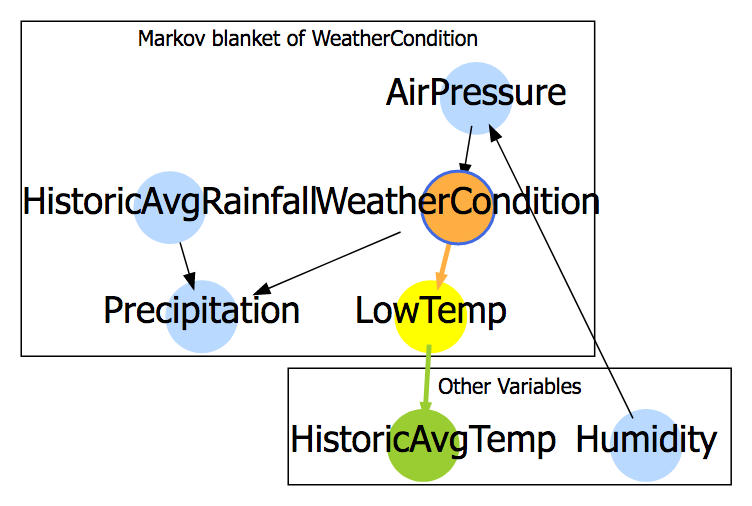
\includegraphics[width=1\textwidth]{CausalGraph1}
    \end{minipage}\hfill
    \begin{minipage}{0.5\textwidth}
        \centering
        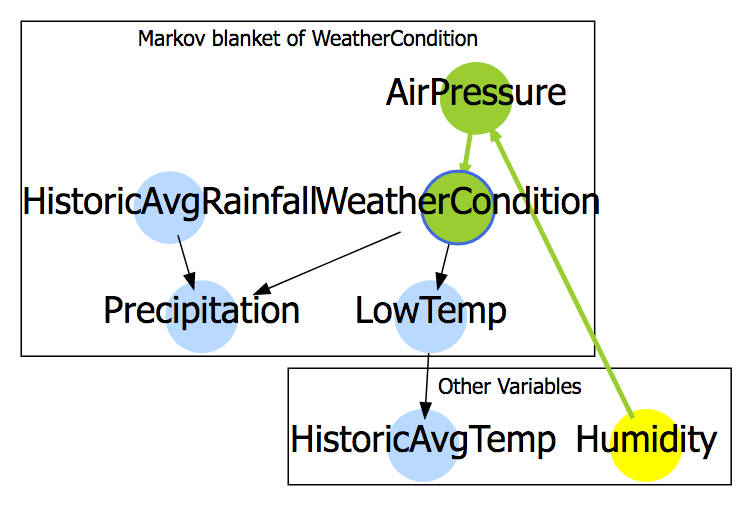
\includegraphics[width=1\textwidth]{CausalGraph2}
    \end{minipage}
    \caption{\textbf{Highlighting Information.} (A) The selected feature is highlighted yellow; direct causes are highlighted orange; direct effects are highlighted green. Low Temperature's Markov blanket consist of a direct cause, weather condition, and a direct effect, Historic Average Temperature. (B) The path to weather condition is highlighted green. Humidity affects weather condition though air pressure.}
    \label{fig:CausalGraphs}
\end{figure}

\subsection{Modifying the Causal Network}
The user can modify the graph to reflect their prior knowledge about the causal relationships between features. For example, the user can remove a feature that the user suspects or believe may not be relevant to the classification task. The feature is removed from the observed data and the causal graph will be rebuilt.

Moreover, the user can remove edges representing relationships that conflict with the user’s prior knowledge and also add new directed edges to represent relationships not captured in the graph. The system prevents the user from adding edges that introduces a cycle. Modifications to the graph may change the Markov blanket features of the target, and consequently, the graph will update to reflect the new information. Graph modifications can be undone and the graph will be reverted.

Initially, the possible graph edits are edge addition, edge removal, and feature removal. We observed during the pilot of the evaluation study that participants made many edges reversals. In order to reverse an edge, they first remove an edge $X \rightarrow Y$, let the graph update, and then add a new edge $Y \rightarrow X$. We added edge reversal as a fourth possible graph edit in order to condense a two-step edge reversal to one step.

\subsection{Markov blanket (MB) Consistency Score} \label{MBConsistencySubsection}
The Markov blanket consistency score is another metric used for measuring the consistency of the feature set to the prior knowledge. The MB consistency score measures the consistency of the feature set in relation to the causal relationships established. As described in subsection \ref{MarbovBlanket}, a node's Markov blanket variables cut it off from the influence of other variables in the network and are predictive of the node. To stay consistent with the idea that the Markov blanket is predictive, the consistency of the selected features to the target's Markov blanket is calculated. MB score is the fraction of the Markov features that are “covered” by a subset of the selected feature set. A Markov blanket feature is “covered” if a subset of the selected features form a connected path to the feature or is a selected feature. Let \(B\) be the set of Markov blanket features, the MB Score is expressed as

\begin{equation}
\label{eqn:MBConsistency}
MB Score = 
\sum_{f \in B}
    \begin{cases}
      1/|B| & \text{if f is covered}\\
      0 & \text{otherwise}
    \end{cases} 
\end{equation}

A Markov blanket feature is given the same score as a subset of features that form a connected path to the Markov blanket feature. The user may not want to use a Markov blanket feature for various reasons, such as the feature may be difficult or costly to measure. The user can consider replacing the Markov blanket feature with related features, and there are various ways the user can interact with the graph to find replacements. First, the user can highlight the feature's Markov blanket to identify features that directly influence it. For example, in figure \ref{fig:CausalGraphs}, low temperature is in the target's Markov blanket, and historic average temperature (highlighted in green) is a direct effect of low temperature. We can replace low temperature with historic average temperate in a feature set and low temperate would be covered. Second, the user can also highlight connected paths between a feature and target. For example in figure \ref{fig:CausalGraphs}, humidity has a path to weather conditions through air pressure. We can replace air pressure with humidity in a feature selection, and air pressure would still be covered. 

\section{Exploring Feature Space}
\begin{figure}[!htbp]
\centering
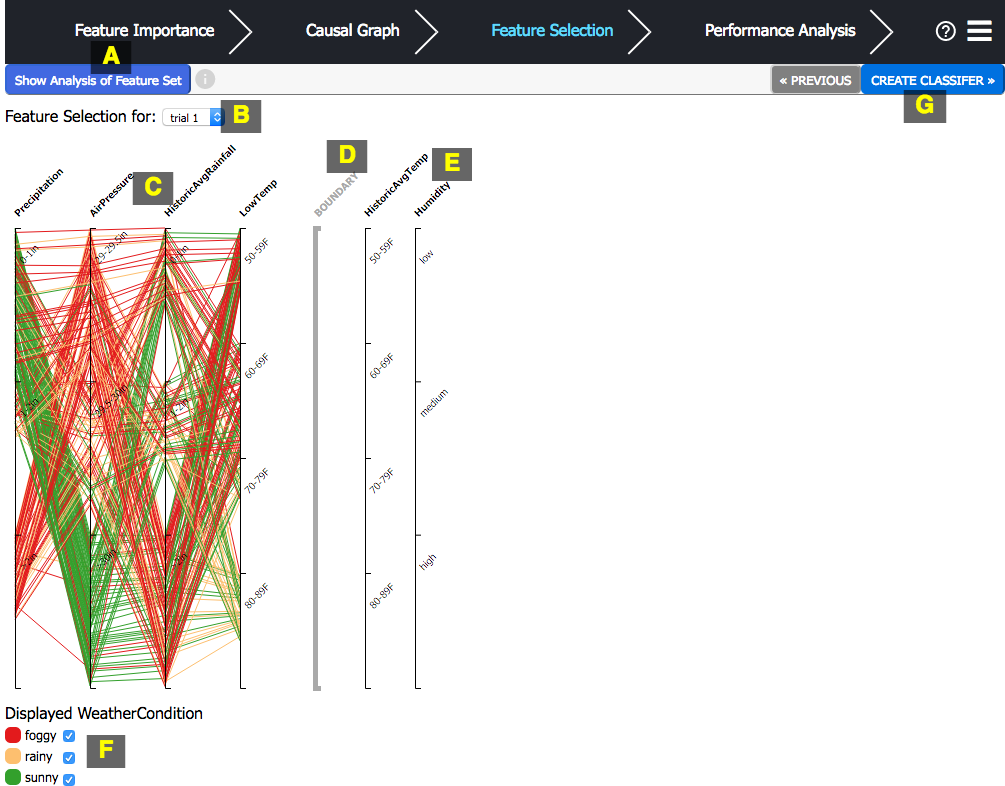
\includegraphics[width=1\textwidth]{LabeledFSInterface}
\caption{\textbf{Exploring Feature Sets Interface.} (A) Click ``Show Analysis of Feature Set" to switch to the analysis view. The analysis view is used to evaluate current feature selection against previously established prior knowledge. (B) The user can select to display the feature selection for previously trained models. (C) Features are represented as vertical axes. Features to the left of the BOUNDARY axis are in the selected feature set. Each line represents an example and intersects a feature axis at the feature value for that example. The line color corresponds to the target label of the example. (D) The BOUNDARY axis separates the selected features on its left from the not selected features on its right. (E) Lines representing examples do not extend beyond the BOUNDARY axis to the feature axes that are not selected. (F) The legend correlates color to target label. The user can also select which target labels to be displayed on the interface. } \label{fig:LabelFSInterface}
\end{figure}

After feature importance and causal relationships have been established, the user explores possible feature sets. We designed the feature selection interface to support interactive exploration of the feature space, to identify patterns in the dataset, and to evaluate the consistency of a feature set in relation to prior knowledge. Components are designed to communicate information about features. Prior knowledge is integrated to help the user filter features. The interactions are designed to support the efficient exploration of feature space and comparison of feature sets. 

The design of the feature selection interface and interactions also attempts to prevent overfitting. We enable the user are able to utilize their prior knowledge and the visual components for describing prior knowledge discussed in the later section to manual select predictive features and filter out not predictive features. As opposed to the common feature selection methods that limit the control of the user at selecting features, the user can easily add or remove features from the selected feature set based on information about feature importance and causality and help the system prevent overfitting.   

A feature is represented as a vertical axis, identified by the feature name at the top of the axis. A continuous feature axis ranges from the minimum to the maximum feature value. A discrete feature axis is equally partitioned into its feature values. The BOUNDARY axis separates the selected features on its left from the not selected features on its right as shown in figure \ref{fig:FSCorrelation}. 

The default feature set is the target's Markov blanket, which is consistent with the previously expressed information and has a Markov blanket consistency score of 1.0. A default model is created using the target's Markov blanket features and labeled as the trial 0 model. The user can compare the consistency of a feature set and performance of a model against the default model and should attempt to create a model that performs better. 

\subsection{Displaying Examples}
Examples are incorporated into the visual to identify patterns between feature values and target labels. Each example is represented by a line. The color of the line corresponds to the target label of the example. The line intersects a selected feature axis at the example's feature value and does not extend beyond the BOUNDARY axis to unselected feature axes. For continuous features, the line intersects the continuous axis at the feature value. For discrete features where a partition of the axis corresponds to a value, the line intersects the next available point in the value partition. Discrete feature values are a partition of the axes rather than a point to prevent many lines from converging at a specific value on the axis which may mislead the user on how many examples are represented by the line. Separating the examples with the same discrete feature value also helps better identify patterns and correlations between feature values. 

\subsection{Interactive Feature Selection}
The interface is designed to enable the user to interactively select features. Features can be added or removed from the selected feature set by dragging the feature axis to the left of the boundary or right of the boundary, respectively. Moreover, the boundary axis can also be dragged so that features to its left are selected and features to its right are not selected. The visualization enables users to interactively and quickly select a feature set and efficiently make elementary modifications to the feature selection. This helps the user efficiently explore and analyze different feature sets. The graph dynamically updates after a feature axis is repositioned. Other visual components and calculations that depend on the selected feature set also dynamically update. Features can be repositioned to help identify patterns or correlations. For example, figure \ref{fig:FSCorrelation} shows the correlation between feature values in the first axis, Air Pressure, and feature values in the second axis, Humidity. Examples with air pressure greater than 30in are likely to have a medium level of humidity. 

\begin{figure}[!htbp]
\centering
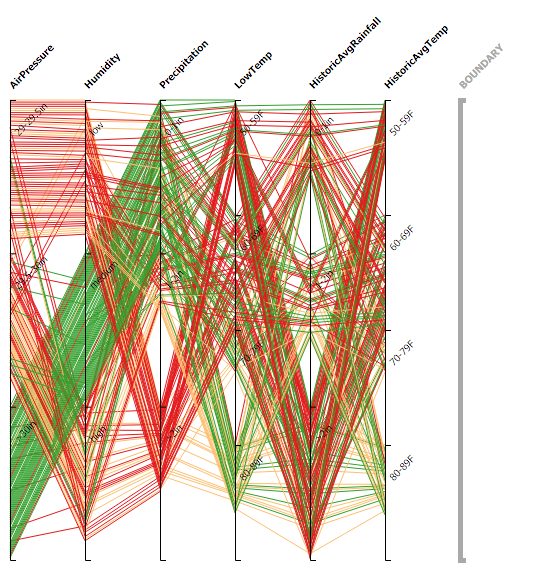
\includegraphics[width=0.65\textwidth]{FSCorrelation}
\caption{\textbf{Correlation Between Features.} Air pressure is correlated to humidity. Examples with air pressure greater than 30in is highly likely to have medium level of humidity, while examples with air pressure between 29-29.5in is more likely to have low level humidity} \label{fig:FSCorrelation}
\end{figure}

\subsection{Filtering Visual Information}
Filtering functionalities are implemented to allow the user to reduce the amount of visual information and better identify patterns. First, the user can select and deselect which target labels to display. When a target label is deselected, the graph dynamically updates the color of unselected examples to a light gray. Skewed datasets can be detected since the color of the dominating target label will dominate the graph. Another benefit of filtering is that the user can filter out dominating target labels and focus on the less frequent target labels. Moreover, filtering for a specific target label can help the user visually identify feature values that are related to that target label \ref{fig:FilterTargetLabel}.

\begin{figure}
    \centering
    \begin{minipage}{0.7\textwidth}
        \centering
        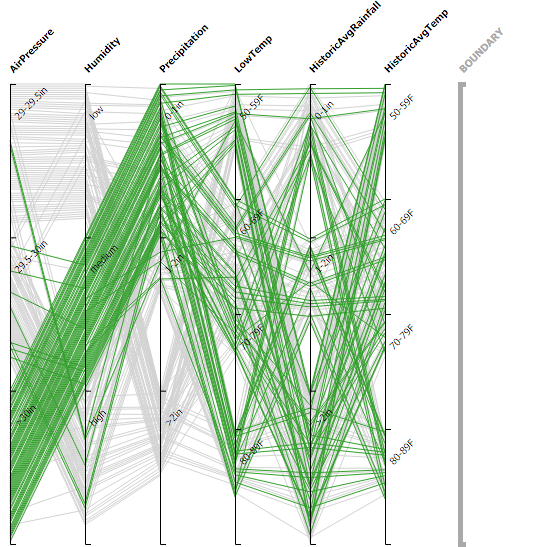
\includegraphics[width=.85\textwidth]{FilterTargetLabel}
    \end{minipage}\hfill
    \begin{minipage}{0.3\textwidth}
        \centering
        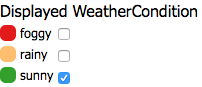
\includegraphics[width=1\textwidth]{FilterTargetLabelLegend}
    \end{minipage}
    \caption{\textbf{Filter Target Label}. User filtered for sunny examples/days. The visual shows that greater than 30 in air pressure, medium (30-60\%) humidity, and 0-1in precipitation are weather metrics that are correlated to tomorrow's sunny weather condition.}
    \label{fig:FilterTargetLabel}
\end{figure}

In addition, the user can filter for feature values by highlighting a range in the feature axis. Feature ranges can be highlighted for multiple feature axes. The entire feature range is used by default for features without a specified filter range. Each time a filter is updated, the graph dynamically grays the lines representing examples whose feature values are not in all of the specified feature ranges. Filtering for feature value can help the user visually identify patterns. For example, in figure \ref{fig:FilterTargetLabel}, after the user had filtered out rainy and foggy examples, the graph reveals that most of the sunny examples have precipitation between 0 and 1 inch the previous day. Filtering by feature values can also help identify which sets of feature values may distinguish a target label as shown in figure \ref{fig:FilterValues}.

\begin{figure}[!htbp]
    \centering
    \begin{minipage}{0.7\textwidth}
        \centering
        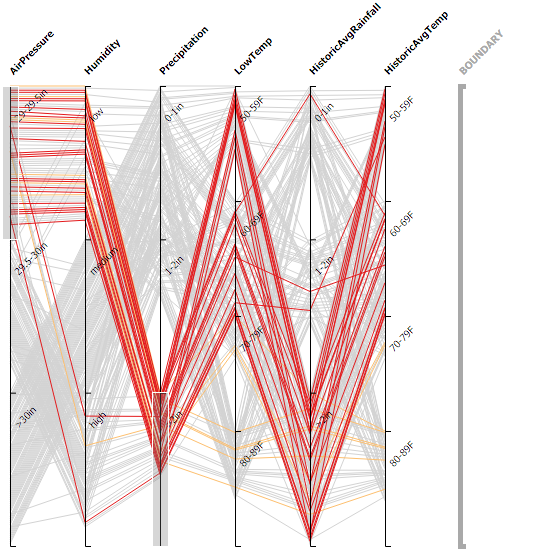
\includegraphics[width=.85\textwidth]{FilterValues}
    \end{minipage}\hfill
    \begin{minipage}{0.3\textwidth}
        \centering
        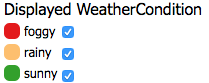
\includegraphics[width=1\textwidth]{FilterValuesLegend}
    \end{minipage}
    \caption{\textbf{Filter Feature Values}. User filters for examples/days with air pressure between 29.0 and 29.5in and precipitation of greater than 2 in. The interface reveals that examples with both these metrics are more likely to have foggy weather conditions.}
    \label{fig:FilterValues}
\end{figure}

\begin{figure}[!htbp]
\centering
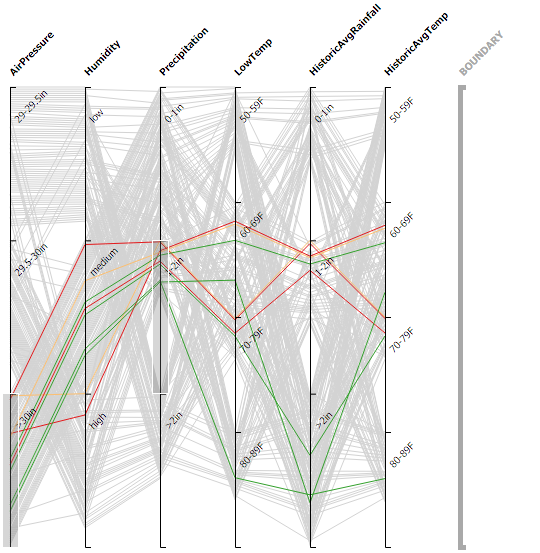
\includegraphics[width=0.65\textwidth]{FilterValuesSparse}
\caption{\textbf{Uncorrelated Feature Values}. User filtered for examples/days with air pressure greater than 30.0in and precipitation between 1 to 2in. All possible target labels are represented in the few examples that are unfiltered, which reveals that these two feature values are most likely uncorrelated or rarely occur together.} \label{fig:FilterValuesSparse}
\end{figure}

\subsection{Metrics for Analyzing Feature Set}
\begin{figure}[!htbp]
\centering
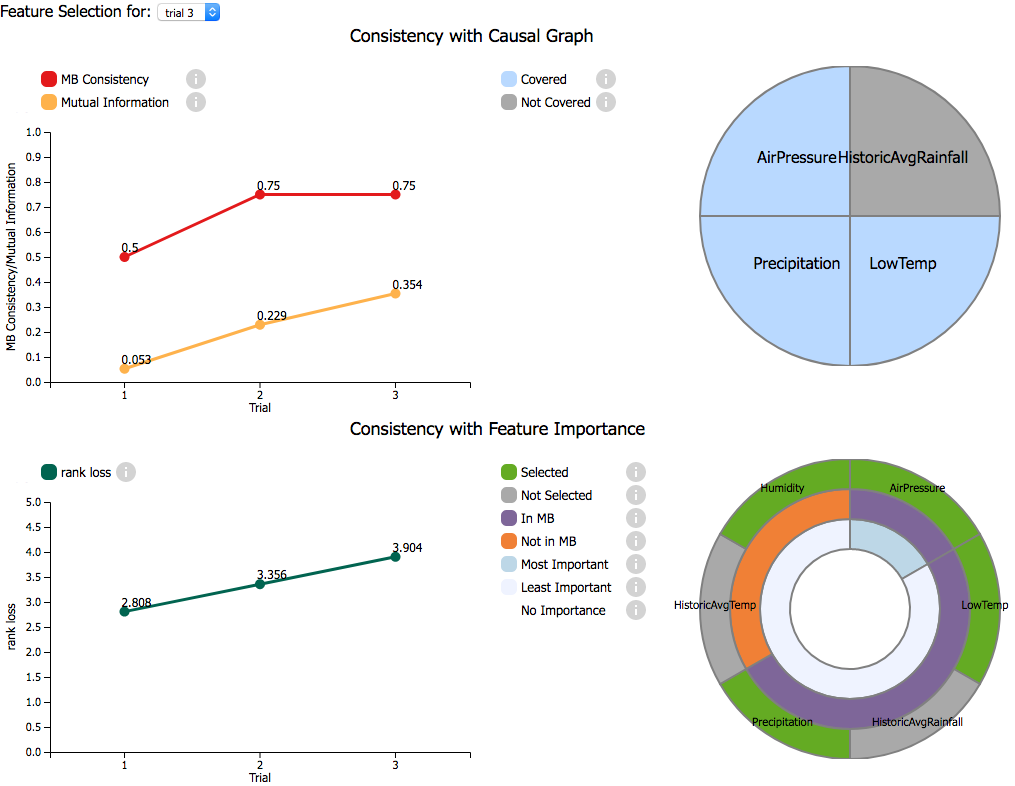
\includegraphics[width=1\textwidth]{FeatureAnalysisInterface}
\caption{\textbf{Feature Selection Analysis Interface.} At the feature selection step, user can switch to the analysis view to assess metrics and graphs that help determine whether the current feature set is a good choice and whether it is consistent to the user's prior knowledge.} \label{fig:FeatureAnalysisInterface}
\end{figure}

Metrics are calculated to describe how consistent a feature set is to feature importance and causalities expressed in previous steps. Scores are dynamically calculated and updated each time the feature selection changes. The three metrics calculated are Markov blanket (MB) consistency score, mutual information (MI) score, and rank loss.

\subsubsection{Markov Blanket Consistency Score and Coverage Pie Chart}
The MB score describes the feature set consistency in relation to causalities expressed in the Bayesian network build in the previous step. Refer to section \ref{MBConsistencySubsection} and equation \ref{eqn:MBConsistency} for the MB score calculation. The MB score has a range of [0.0, 1.0], where 1.0 corresponds to all features being covered and 0.0 corresponds to none of the features being covered. The default feature selection with the Markov blanket features has a score of 1.0. The feature set that maximizes the Markov blanket score is not unique. The user can attempt to maximize the score to stay consistent with established prior knowledge.

In complementary to the score, a pie chart visually shows which Markov blanket features are covered as shown in figure \ref{fig:CoverageChart}. The pie chart is equally divided into slices that correspond to the set of Markov blanket features. Covered features are highlighted blue, while uncovered features are highlighted gray. The fraction of blue on the chart corresponds MB score that reports the fraction of covered features. Since the score and chart are dependent on the previously provided information, modification to the causal graph will cause the pie chart to update with the new Markov blanket features and the score to be recalculated.

\begin{figure}[!htbp]
    \centering
    \begin{minipage}{0.5\textwidth}
        \centering
        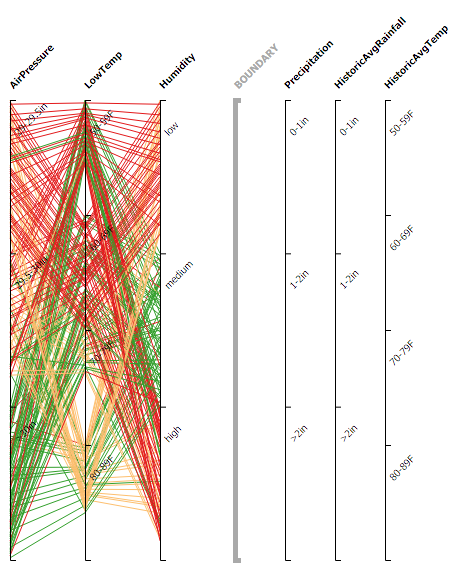
\includegraphics[width=1\textwidth]{SelectedFeaturesCoverage}
    \end{minipage}\hfill
    \begin{minipage}{0.5\textwidth}
        \centering
        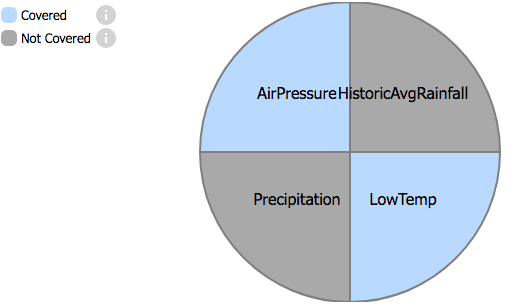
\includegraphics[width=1\textwidth]{CoverageChart}
    \end{minipage}
    \caption{\textbf{Markov Blanket Feature Coverage Chart.} The chart is composed of the four features that make up the target's Markov blanket. Air pressure and low temperature are in the selected set and are covered, while precipitation and historic average rainfall are not in the selected set and are not covered. } \label{fig:CoverageChart}
\end{figure}

\subsection{Mutual Information (MI) Score}
The MI score is computed using Mutual Information Maximization (MIM) scoring criterion \ref{eqn:MIM}, which can use as a criterion in filter-based feature selection methods. Mutual information is a measure of the amount of information that one random variable has about another random variable. The mutual information between two independent features is 0. The MIM score expresses the sum of the information shared between the selected features and the target in terms of entropy. The MI score can also support users at filtering features. For example, if the addition of a feature increases the MI score significant, then the feature has information about the target. On the flip side, if the score does not increase by much, then the feature does not have much information about the target. However, MIM does not account for the redundant information a feature has about the target that may already be accounted for by another feature in the selection. 
A mutual information score is incorporated in the analysis because information measure based metrics are commonly used to filter for features, and therefore can be used for assessing the feature selection. The MI score is calculated as an additional predictor of whether the selected feature set will result in a high performing model. MIM function can be replaced by other mutual information functions or more mutual information scores can be incorporated into the interface. 

\subsection{Rank Loss and Feature Importance Consistency Chart}
\begin{figure}[!htbp]
\centering
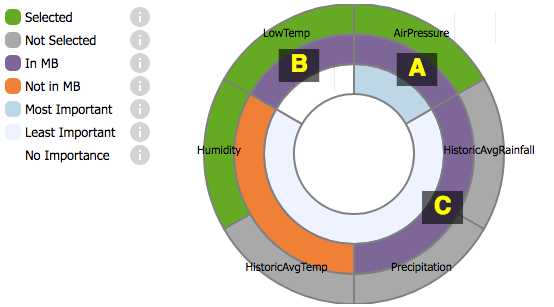
\includegraphics[width=0.75\textwidth]{SunburstChartLabeled}
\caption{\textbf{Feature Importance Consistency Chart.} (A) Air Pressure is the most important feature and is part of the feature selection. (B) However, Low Temp, the least important feature is also apart of the feature selection. (C) Half of the Markov blanket features are not included in the feature selection.} \label{fig:SunburstChart}
\end{figure}
Rank loss \ref{eqn:rankloss} expresses the consistency the feature set to the expressed feature importance. The minimum value of rank loss is 0. A feature selection that is consistent with feature importance minimizes rank loss. 

A complementary chart is designed to visually express the consistency of the feature selection to the feature importance information. The chart is a sunburst or multilevel pie chart used to encompass various levels of information. The outermost pie is equally divided into all the features. The second pie shows whether the adjacent feature in the outer circle is in the target's Markov blanket or not. Markov blanket features are filled in purple and non-Markov blanket features in orange. Lastly, innermost pie describes the importance of the adjacent feature - the color of the slice corresponds to the color of the circle the feature was grouped in during the feature importance step. 
In the outer circle, the features that are filled in green are part of the feature selection while the features filled in gray are not. By organizing the information in a multilevel fashion, the user can see if the more important features are included in the feature selection and also if Markov blanket features are relatively important.

\subsection{Progress Graphs}
\begin{figure}[!htbp]
    \centering
    \begin{minipage}{0.5\textwidth}
        \centering
        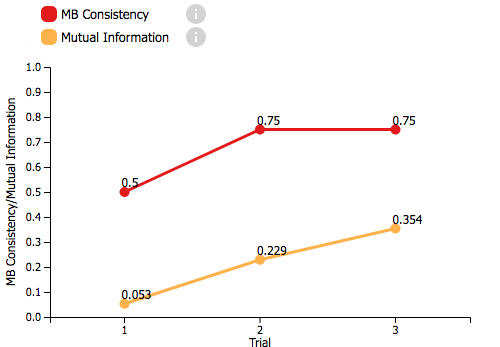
\includegraphics[width=1\textwidth]{MIGraph}
    \end{minipage}\hfill
    \begin{minipage}{0.5\textwidth}
        \centering
        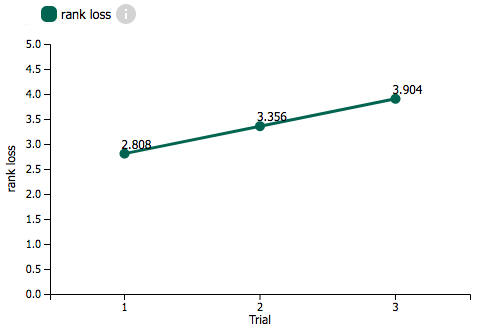
\includegraphics[width=1\textwidth]{RankLossGraph}
    \end{minipage}
    \caption{\textbf{Progress Graphs.} Metrics are used to assess whether the feature set may produce a high performing model and how consistent the feature set is to previously provided information. Metrics are calculated for each model and plotted to show the progress in model construction. MB consistency scores of the feature sets have increased since the first iteration, so more Markov features are covered in the later iterations. MI score has also increased, so the amount of shared information between selected features and target has increased. } \label{fig:ProgressGraph}
\end{figure}
The system enables the user to iteratively construct models. The progress of the models' metrics is tracked. The MB and MI scores are displayed in one graph and the rank loss score is displayed in a separate graph because maximizing the MB and MI scores corresponds to an increase in consistency while minimizing the rank loss score corresponds to an increase in consistency. Initially, the graphs only display the metrics for the first trial. The scores for the current feature selection dynamically update when the feature set updates. 

The system is designed for the iterative model building process. A model is built with the current feature selection. The user can continue to build models with different feature sets. A model is constructed at each iteration, which is labeled as a trial in the system. The information pertaining to previous trials, such as selected features, metrics, and model performance, is retained for the purposes of comparing and contrasting the models. The metrics for analyzing feature sets are displayed as a line graph to display the progress of the model creation process and also to compare the metrics of the different trials.  

\subsection { Classification Algorithm }
The system builds a model from the user selected features - the features on the left of the BOUNDARY axis. A basic classification algorithm is used to create the model. For the evaluation study, we use the k-nearest neighbors algorithm (kNN) for classification and set the number of nearest neighbors $k$ to use as 3. The kNN algorithm assigns an example to the target label that is most common among its $k$ nearest neighbors. The interactive feature selection system is designed to be model agnostic. In theory, the user will be able to specify the classification algorithm and its input parameters. The feature for allowing the user to pick the classifier and its parameters directly from the user interface has not been implemented.

Moreover, we perform stratified $k$ fold cross validation to access the accuracy and performance of the resulting classifier. The original dataset is randomly partitioned into $k$ equal sized subsets where the fractions of target labels equal that of the original data set. Of the $k$ subset, a single set is retained for testing the resulting classifier; the remaining $k-1$ sets are used as training data to create the classifier. The cross-validation process is repeated $k$ times. Each of the subsets is used once as testing data. Lastly, the $k$ results such as test accuracy is averaged to produce the overall test accuracy.

\subsection{Performance Analysis} \label{PASection}
The system incorporates performance analysis to assess the model. The user is automatically taken to the performance analysis interface after a model is built. Accuracy, the percentage of the examples whose target labels are correctly predicted, is a commonly used metric to assess a model's performance and is used at this step. 

Another component of the interface is the confusion matrix, which is a commonly used table for reporting classification results. The rows of the matrix correspond to the actual labels and the columns correspond to the model's predicted labels of the example. The matrix communicates how many examples of a label are predicted as the other target labels. A high performing model will have a high concentration of examples along the diagonal - as those cells correspond to how many examples of a label are correctly predicted as that label. However, because the dataset can be skewed towards a certain target label, the magnitude of the numbers along the diagonal may bias the viewer's assessment of the model's performance. To provide more information, the cells of the confusion matrix are colored using an orange color scale. The scale mapped to the accuracy range 0.0 to 1.0, where the lightest orange correlates to 0.0 and the darkest orange correlates to 1.0. The color represented the fraction of examples of a target label that are predicted as the target label corresponding to the column. A high performing model that correctly predicts examples has the darkest orange along the diagonal and light orange everywhere else. 

\begin{figure}[!htbp]
\centering
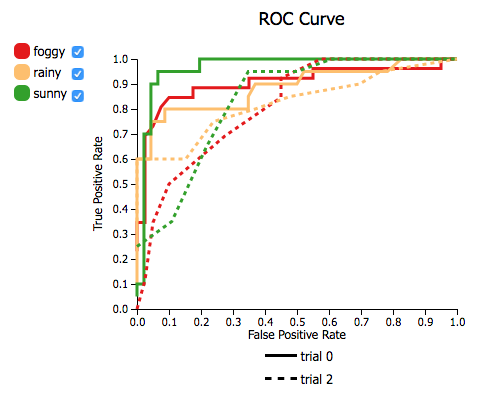
\includegraphics[width=0.75\textwidth]{ROCmultiple}
\caption{\textbf{ROC Curves.} The ROC curves for trial 0 and trial 3 models are plotted as solid and dotted lines respectively. The user can select to display the curves of certain target labels. A greater area under the ROC curve represents higher performance. By overlaying ROC curves of two models, we can see which curve has a greater area under the curve and determine which model performs better.} \label{fig:ROCmultiple}
\end{figure}

Receiver operating characteristic (ROC) curves are used for visual performance analysis. The ROC curve is created by plotting the true positive rate against the false positive rate at various probability thresholds. The model often provides confidence scores for their predictions - for example, the model may be 67\% certain that this example's weather condition is sunny. The probability threshold, a parameter often set by the user, is how certain the model has to be before it can make its prediction. 
For classification problems where there are three or more possible labels, an ROC curve is plotted for each of the labels. Each curve plots the rate the model correctly predicts examples of that label against the rate the model incorrectly predicts the examples as any of the other labels as shown in figure \ref{fig:ROCmultiple}. The area under the curve (AUC) is an indicator or the model's performance. A greater area under the curve represents higher performance. 

\begin{figure}[!htbp]
\centering
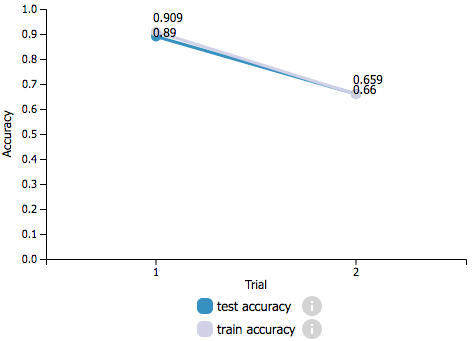
\includegraphics[width=0.75\textwidth]{accuracy}
\caption{\textbf{Accuracy Graph.} The training and testing accuracy of each iteration are plotted to show the progress and to compare models. Training accuracy is the fraction of examples in the training set that the model correctly predicted; testing accuracy is the fraction of unseen examples that the model correctly predicted. In this figure, the first trial has greater training and testing accuracy than the second trial. } \label{fig:accuracy}
\end{figure}

\subsection{Comparing Models}
\begin{figure}[!htbp]
\centering
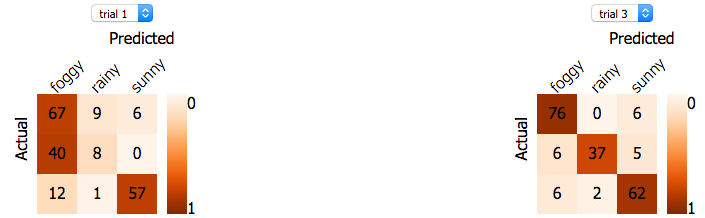
\includegraphics[width=1\textwidth]{ConfusionMatrixCompare}
\caption{\textbf{Comparing Model Performances.} We compare the third model with an accuracy of 0.87 against the first model with an accuracy of 0.66. The third model's confusion matrix has darker orange along the diagonal, which indicates it has a higher percentage of correctly predicted examples for each of the target labels. On the other hand, the first model's confusion matrix shows that its confusing many rainy examples for foggy examples. } \label{fig:ConfusionMatrixCompare}
\end{figure}

\begin{figure}[!htbp]
\centering
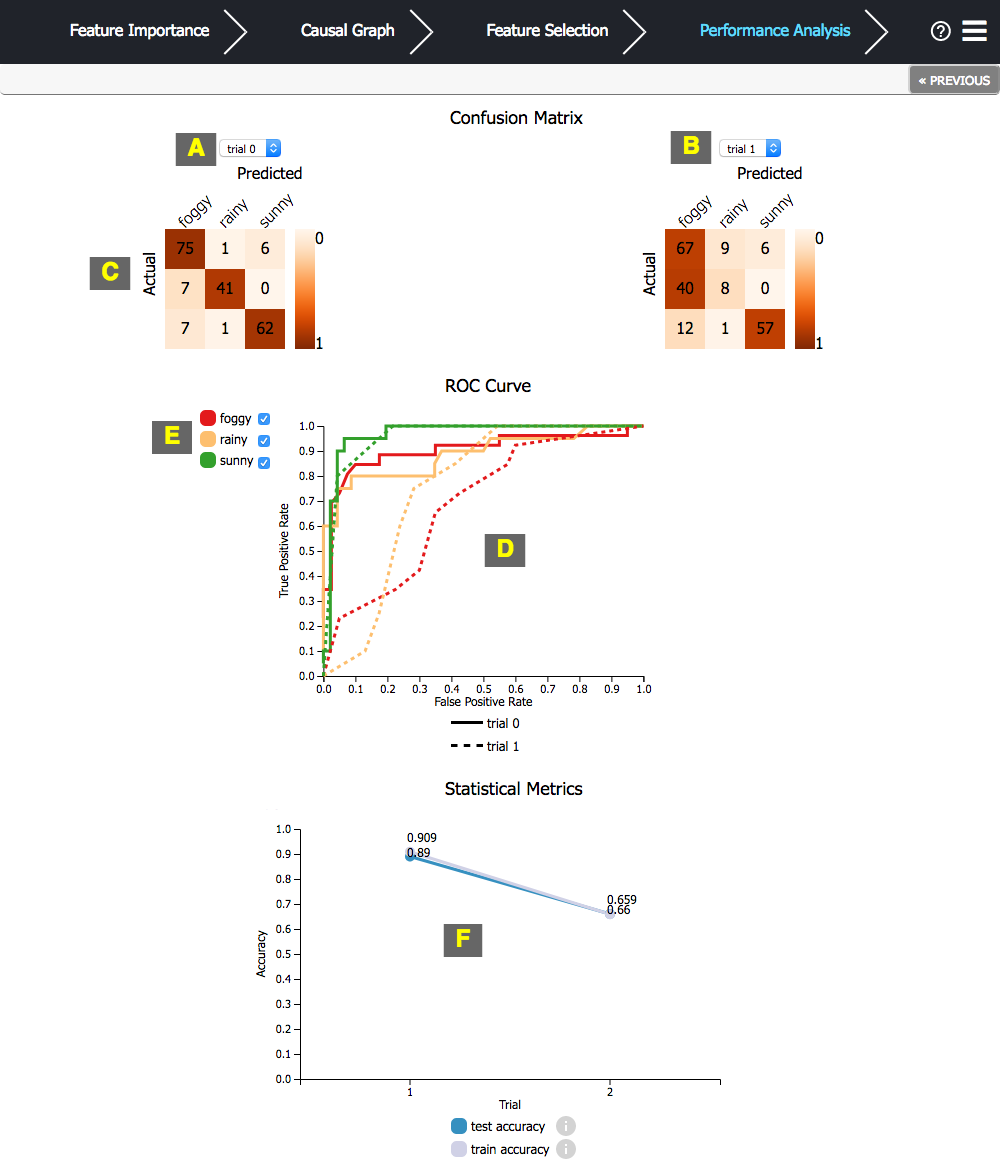
\includegraphics[width=1\textwidth]{compareclassifierspageview}
\caption{\textbf{Comparing Model Performances.} We compare the third model with an accuracy of 0.87 against the first model with an accuracy of 0.66. The third model's confusion matrix has darker orange along the diagonal, which indicates it has a higher percentage of correctly predicted examples for each of the target labels. On the other hand, the first model's confusion matrix shows that its confusing many rainy examples for foggy examples. } \label{fig:PerformanceAnalysisPage}
\end{figure}

The performance analysis step is designed for iterative model creation. Training and testing accuracies are displayed in a line graph to show the progress of the model creation process. The graph can also be used to compare the accuracy of different models. Moreover, two confusion matrices are shown side by side for the purpose of comparison. By default, when a new model is created, the left confusion matrix is updated to display performance of the newest created model and the right matrix is updated to display the previous model created. The user can choose which trial's confusion matrix to display and which models to compare by selecting the trial to display using the selection element above the confusion matrix, as shown in figure  {fig:PerformanceAnalysisPage}.

The user can also compare model performances using the ROC curve. The user can select which two trials' ROC curves to display. One trial's curves will be in solid while the other's curves will be dotted as shown in figure \ref{fig:ROCmultiple}. Since the area under the curve is an indicator of model performance, ROC curves are well fit for visually comparing performance. By overlaying curves from different models, we can see which model produces curves with larger areas. Moreover, the user can also select which target label's curve they want to be displayed.  

Moreover, the system retains information about previous trials to show which feature sets were already tried. To correlate the performance of the model with the feature set used to create the model, the user set the corresponding trial to display at the feature selection step. Then, the interface for the feature selection step and the graph for assessing the feature set updates to reflect the feature set used for the selected trial. In addition to selecting previously selected feature sets for comparison, the user can also select high performing iterations and make changes to that feature set in attempt to create a higher performing classifier. This function is used by participants during the user study to improve on previously selected feature sets. The interface and interactions are designed to enable the user to compare and contrast models and visually keep track of their model creation progress. They help with the iterative nature of the classification progress by showing the progress of the iterations, retaining information about the previous iterations, and enabling the user to access feature sets from previous trials and then modified the original feature set. 

